% ------------------------- MAIN TASK ---------------------------------
\section{Développement schématique}

\clearpage
\subsection{Choix des composants} \label{ssec:num32}
{
	\subsubsection{Microcontrôleur}
	Lors de la recherche de composants, j'ai décidé d'utiliser l'un des PIC32 standards de l'ES :
	\textbf{PIC32MX130F064D-I/PT}.
		
	\begin{figure}[h]
		\centering
		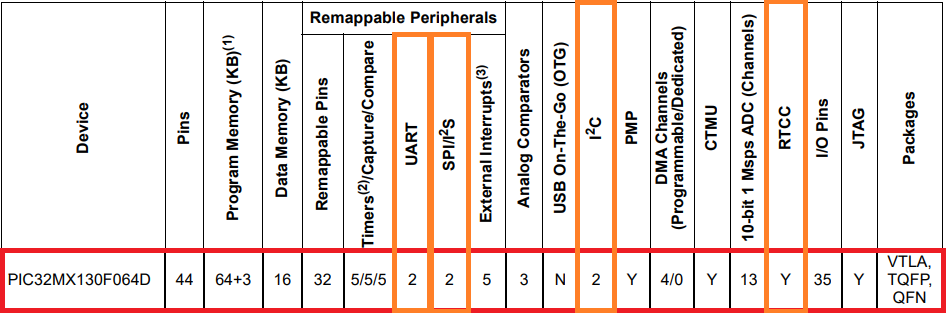
\includegraphics[width=1\linewidth]{Figures/Dev-SCH/PIC32-choisi}
		\caption{Périphèriques disponnibles du PIC}
		\label{fig:pic32-choisi}
		\source{PIC32MM0256GPM064 family datasheet}
	\end{figure}
	
	Nous pouvons constater sur la figure \ref{fig:pic32-choisi} que les critères minimaux de mon projet sont respectés :
	
	\begin{center}
		\fbox{\textit{1 - I2C}} \fbox{\textit{1 - SPI}} \fbox{\textit{1 - UART}} \fbox{\textit{1 - RTCC}}
	\end{center}
\subsection{Dimensionnements} \label{ssec:num31}
{}
}
\subsection{Oscillogram of the output current depending on the input tension} \label{ssec:num33}
{}
\subsection{Dissipated power calculation} \label{ssec:num34}
{}
\subsection{Estimation of the junction's temperature without cooling} \label{ssec:num35}
{}
\subsection{Short-circuited output - dissipated power calculation} \label{ssec:num36}
{}
\clearpage